% !TeX root = ../main.tex

\chapter{研究背景}
\label{chap:background}
本章我们将系统的分析本项目的研究背景以及相关知识,并且分析现有工作已经取得的成果与不足。本章将从排序算法简介、软硬件协同设计综述、FPGA与高层次综合综述、相关研究等四个方面进行介绍。
\section{排序算法简介}

排序算法一直是一个热门的研究问题,即使其问题表述非常简单,但是人们一直期盼能够找到更加高效的排序算法。早在1951年,Betty Holberton就开始着力解决排序算法问题;在1956年,Howard提出了冒泡排序算法\cite{demuth1956report}。在此之后,新算法层出不穷,有些算法如Timsort\cite{mcilroy1993optimistic}, Library sort\cite{bender2006insertion}等均已经得到了非常广泛的应用。

目前,对于小型数组的快速排序(尽可能少的比较和交换次数)仍然是一个值得研究的问题,同时,在并行系统上如何能够尽可能的提高排序算法的效率,也是一个值得讨论的话题。本课题即希望通过一些算法和架构的优化设计,得到一些解决此问题的启发。


\section{软硬件协同设计综述}
软硬件协同设计是指通过硬件和软件的同时设计,利用它们的协同作用来实现系统级目标\cite{de1997hardware}。软硬件协同设计是一个比较宽泛的概念,但是其核心思想主要为软件层面和硬件层面上的协同优化,从而达到更好的性能。


对于计算机系统,我们可以使用不同的抽象层级来对其进行描述,如图\ref{fig:computer_system_abstract}所示。对于研究人员而言,如果想要提升计算机的性能,我们可以从不同的抽象层次来进行优化:从硬件层面上来说,可以通过使用新兴器件取代传统CMOS器件,设计新的微架构等方式来提升芯片的性能;从软件层面上来说,可以通过采用新的高效的指令集,采用更加优秀的操作系统、编程语言以及算法来提升计算机解决问题的能力。而软硬件协同设计,则是从“跨抽象层次”的角度来看待问题:在优化软件算法的同时考虑到相关的硬件资源问题,即设计“硬件友好型算法”;在设计硬件架构的同时考虑到对应算法的数据流特征,即设计“特定领域的加速器”。二者相互兼顾的好处就是软件层面与硬件层面能够高度融合,从而达到相较于传统算法以及通用处理器(CPU等)更加优异的性能。
\begin{figure}[htbp]
    \centering
    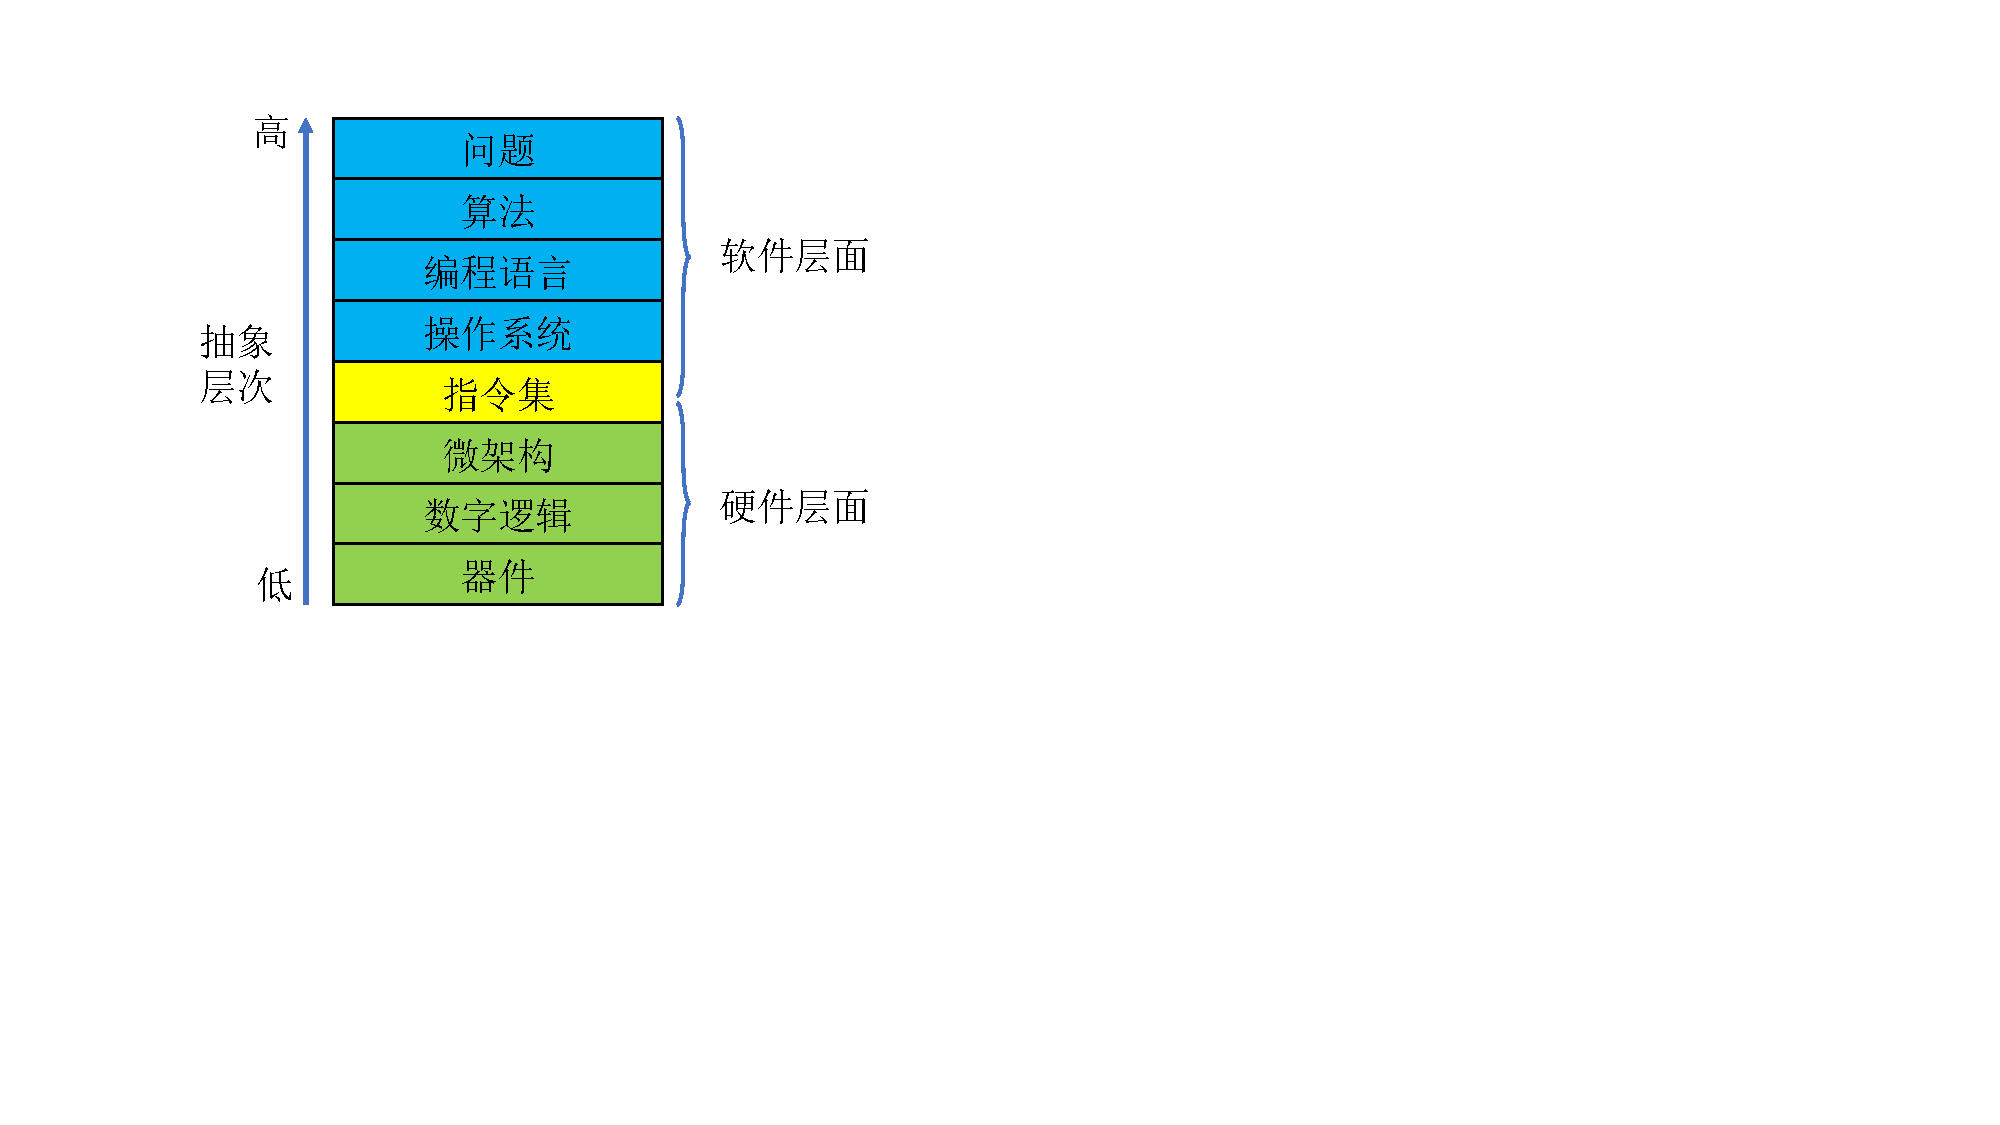
\includegraphics[width=7cm]{figures/computer_system_abstract.pdf}
    \caption{计算机系统的抽象层次示意图}
    \label{fig:computer_system_abstract}
\end{figure}

\section{FPGA与高层次综合(HLS)综述}
\subsection{FPGA简介}
现场可编程逻辑门阵列(Field Programmable Gate Arrays),即FPGA,是一种半定制的集成电路芯片。它可以通过编程来实现几乎任意一种数字逻辑或系统\cite{kuon2008fpga}。与传统的ASIC(Application Specific Integrated Circuit)相比,FPGA可以在不改变硬件电路的情况下进行功能修改,因此更加灵活。 

FPGA由可编程逻辑单元(PL)和可编程输入/输出单元(IO)组成。PL是FPGA的核心部件,它由查找表(LUT)、触发器、多路选择器等多种逻辑门组成,可以通过编程实现不同的逻辑功能。IO单元则提供了FPGA与外部系统的接口,包括数字信号、模拟信号、时钟信号等。FPGA整体架构如图\ref{fig:FPGA}所示。
\begin{figure}
    \centering
    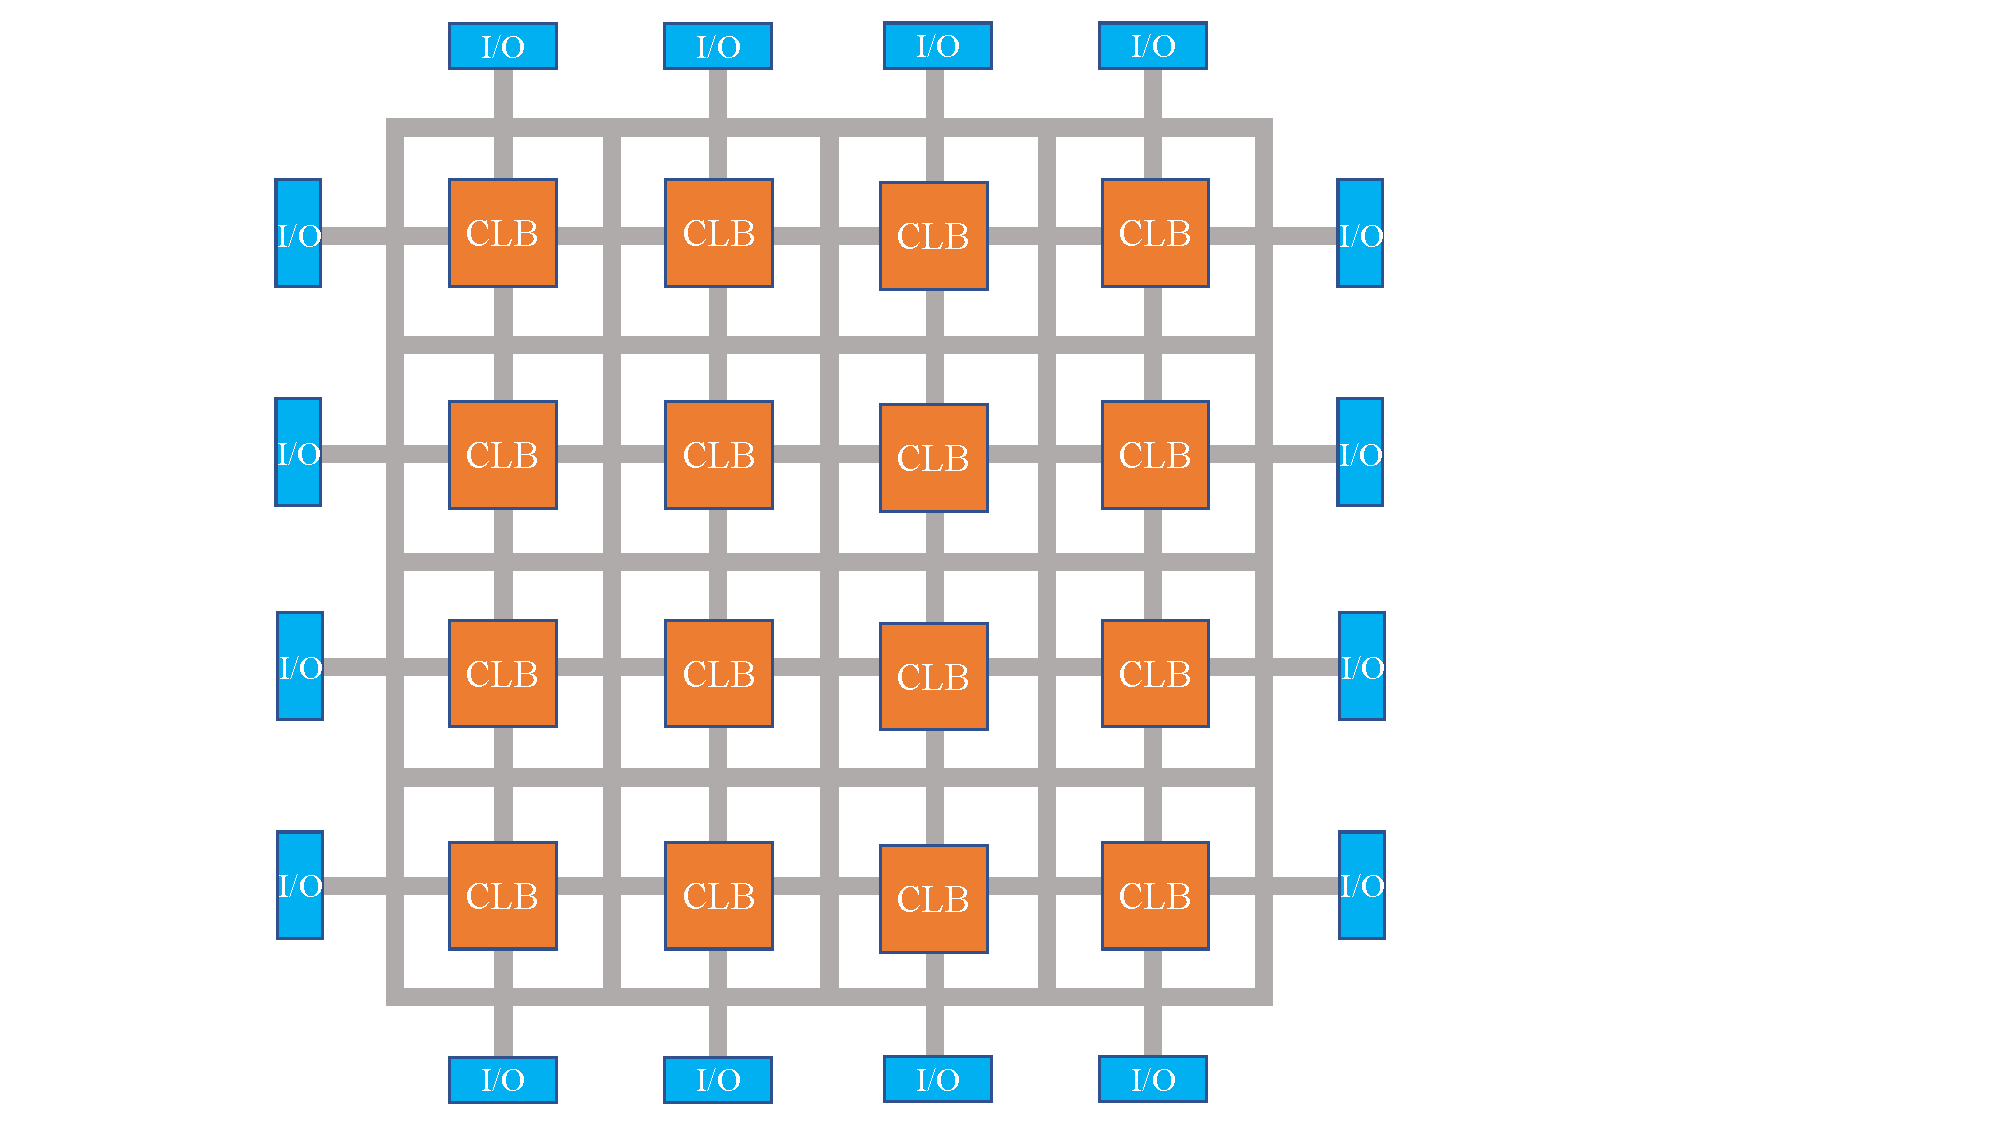
\includegraphics[width=7cm]{figures/FPGA.pdf}
    \caption{FPGA架构示意图}
    \label{fig:FPGA}
\end{figure}

FPGA具有灵活性高、开发周期短、成本低等优点,因此被广泛应用于数字信号处理、控制系统、汽车工业等领域。时至今日,FPGA已经成为数字系统设计中不可或缺的一部分。随着FPGA技术的不断发展,其性能和功能都在不断提升,如今的FPGA不仅支持更高的逻辑密度和更快的工作频率,还可以集成更多的外设和处理器核心。FPGA的高灵活性让其成为设计特定领域加速器(Domain-specific Accelerator)的首选平台。

\subsection{高层次综合简介}

高层次综合(HLS)是一种用于数字系统设计的工具。HLS允许设计人员使用高级编程语言(如C / C ++)来描述数字系统,并自动将其转换为硬件电路。与传统的硬件设计方法相比,HLS具有更快的设计周期和更高的生产效率。

HLS的主要优点之一是可以将抽象的高级语言代码转换为硬件电路,从而减少了设计人员需要了解的硬件细节。这使得设计人员可以更加专注于系统级的设计,而不必担心底层的硬件细节。此外,由于HLS工具可以自动优化设计,因此可以更加轻松的获得拥有更高性能和更低功耗的解决方案。

HLS的发展历程可以追溯到20世纪80年代。当时,人们开始使用高级语言来描述数字系统,但由于计算机性能的限制,这种方法并不实用。2011年,加州大学洛杉矶分校的Jason Cong和康奈尔大学的Zhiru Zhang提出了AutoESL AutoPilot HLS工具\cite{cong2011high},后来被Xilinx收购,成为人们熟知的Vivado/Vitis HLS,大大加速了HLS在科研和实际应用过程中的普及程度。\cite{hlsbook}\cite{pp4fpgas}现在,随着深度学习加速研究的兴起,HLS极大地便利了深度学习加速器的设计,提高了该领域的研究效率。

HLS的未来发展将面临一些挑战。首先,相较于直接编写Verilog,HLS并不能给出最优的硬件架构,即,其给出的方案仍然具有优化空间。另外,在综合编译大型项目的时候,HLS软件的性能仍然需要进一步优化,以Vitis HLS为例,在综合过程中仍然只能利用CPU单核进行处理,这大大限制了HLS工具的性能。\cite{cong2022fpga}但是总的来说,HLS在硬件加速领域仍然具有极为重要的地位,并且具有广阔的发展前景。


\section{排序算法加速的相关研究}

许多研究人员已经对排序算法的硬件加速进行了相关的研究。但是他们的侧重点各不相同。总的来说,他们的研究工作可以通过以下几点来进行分类:
\begin{enumerate}
    \item 选择研究的排序算法,如归并排序,堆排序,基数排序等;
    \item 使用数据集的大小;
    \item 验证平台,如CPU、GPU、FPGA等。
\end{enumerate}

具体来说,Zurek等\cite{zurek2013comparison}比较了不同的并行排序算法在CPU平台和GPU平台上的性能表现;Jan等\cite{jan2012fast}对三种并行排序算法:奇偶排序、等级排序和双调排序算法在CPU和不同GPU架构上的性能进行了比较分析,同时还实现了一种名为min-max蝴蝶网络的新型并行算法,用于在大型数据集中查找最小值和最大值;Konstantinos等\cite{georgopoulos2016evaluation}在FPGA平台上测试了归并排序的性能;Chen等\cite{chen2015energy}对提出了一种新的基于FPGA平台的双调排序算法,使其能够以更高能效、更低延迟运行;Matai等\cite{matai2016resolve}对插入排序进行了优化,并且使用HLS工具对其设计了硬件加速器;Purnomo等\cite{purnomo2016implementation}对冒泡排序进行了并行优化,并在FPGA上面进行了部署。Romanous等\cite{romanous2020high}虽然声称实现了在FPGA平台上实现了对基数排序的加速,但是其方案的具体细节并没有公布;Qiao等\cite{qiao2022topsort}在HBM-FPGA上改进了归并排序,基于存内计算对其实现了加速;Jayaraman等\cite{jayaraman2022hypersort}也基于HBM-FPGA加速了列排序算法;根据上面提供的角度,我们可以对有关研究进行分类,如表\ref{table:previous}所示。
\begin{table}[htbp]
\centering
\caption{相关工作总结}
\resizebox{\linewidth}{!}{
\begin{tabular}{cccc}
\toprule
研究           & 排序算法           & 平台      & 是否通过HLS \\
\midrule
Zurek等\cite{zurek2013comparison}       & 归并排序、双调排序      & CPU、GPU & 否       \\
Jan等\cite{jan2012fast}         & 奇偶排序、等级排序、双调排序 & CPU、GPU & 否       \\
Kostantinos等\cite{georgopoulos2016evaluation} & 归并排序           & FPGA    &  是       \\
Chen等\cite{chen2015energy}        & 双调排序           & FPGA    & 否        \\
Matai等\cite{matai2016resolve}       & 插入排序           & FPGA    & 是       \\
Purnomo等\cite{purnomo2016implementation}       & 冒泡排序           & FPGA    & 否 \\
Romanous等\cite{romanous2020high}     & 基数排序        & FPGA            & 未知  \\
Qiao等\cite{qiao2022topsort}          & 归并排序        & HBM-FPGA        & 否    \\
Jataraman等\cite{jayaraman2022hypersort}  & 列排序      & HBM-FPGA        & 是    \\
\bottomrule
\end{tabular}
}
\label{table:previous}
\end{table}

上述工作虽然对排序算法的优化以及硬件实现进行了探讨,但是他们仍然存在着一定的缺点:
\begin{enumerate}
    \item 部分工作仅仅是在算法层面进行了优化,在硬件架构上并没有讨论,如上述基于CPU、GPU平台的工作\cite{zurek2013comparison, jan2012fast};
    \item 在FPGA平台上的工作仅仅讨论了部分排序算法的优化,且没有对研究成果进行应用,如\cite{georgopoulos2016evaluation,chen2015energy, matai2016resolve, purnomo2016implementation};
    \item 大部分工作并没有发挥HLS的优势,而是使用传统的方式(如Verilog)等进行设计,如\cite{chen2015energy, purnomo2016implementation};
\end{enumerate}

基于以上的原因,我们的工作有以下优点:
\begin{enumerate}
    \item 充分体现软硬件协同设计的思想,即从软件算法角度和硬件加速角度进行了协同优化;
    \item 探究了多种排序算法,同时以尽可能充分利用硬件资源为指导原则,充分发掘各个算法的效率和并行性;
    \item 通过HLS来设计硬件加速架构,更加直观高效。
    \item 将设计的硬件加速架构应用到了解决实际问题当中,在这里我们以八叉树构建过程举例,直观地展示了加速器的加速效率。
\end{enumerate}


